\documentclass{article} % say 
\usepackage[paperheight=2048px,paperwidth=2048px,left=-15px,right=-10px,top=0px,bottom=0px,showframe]{geometry}
\usepackage{tikz}
\usetikzlibrary{backgrounds}
\begin{document}

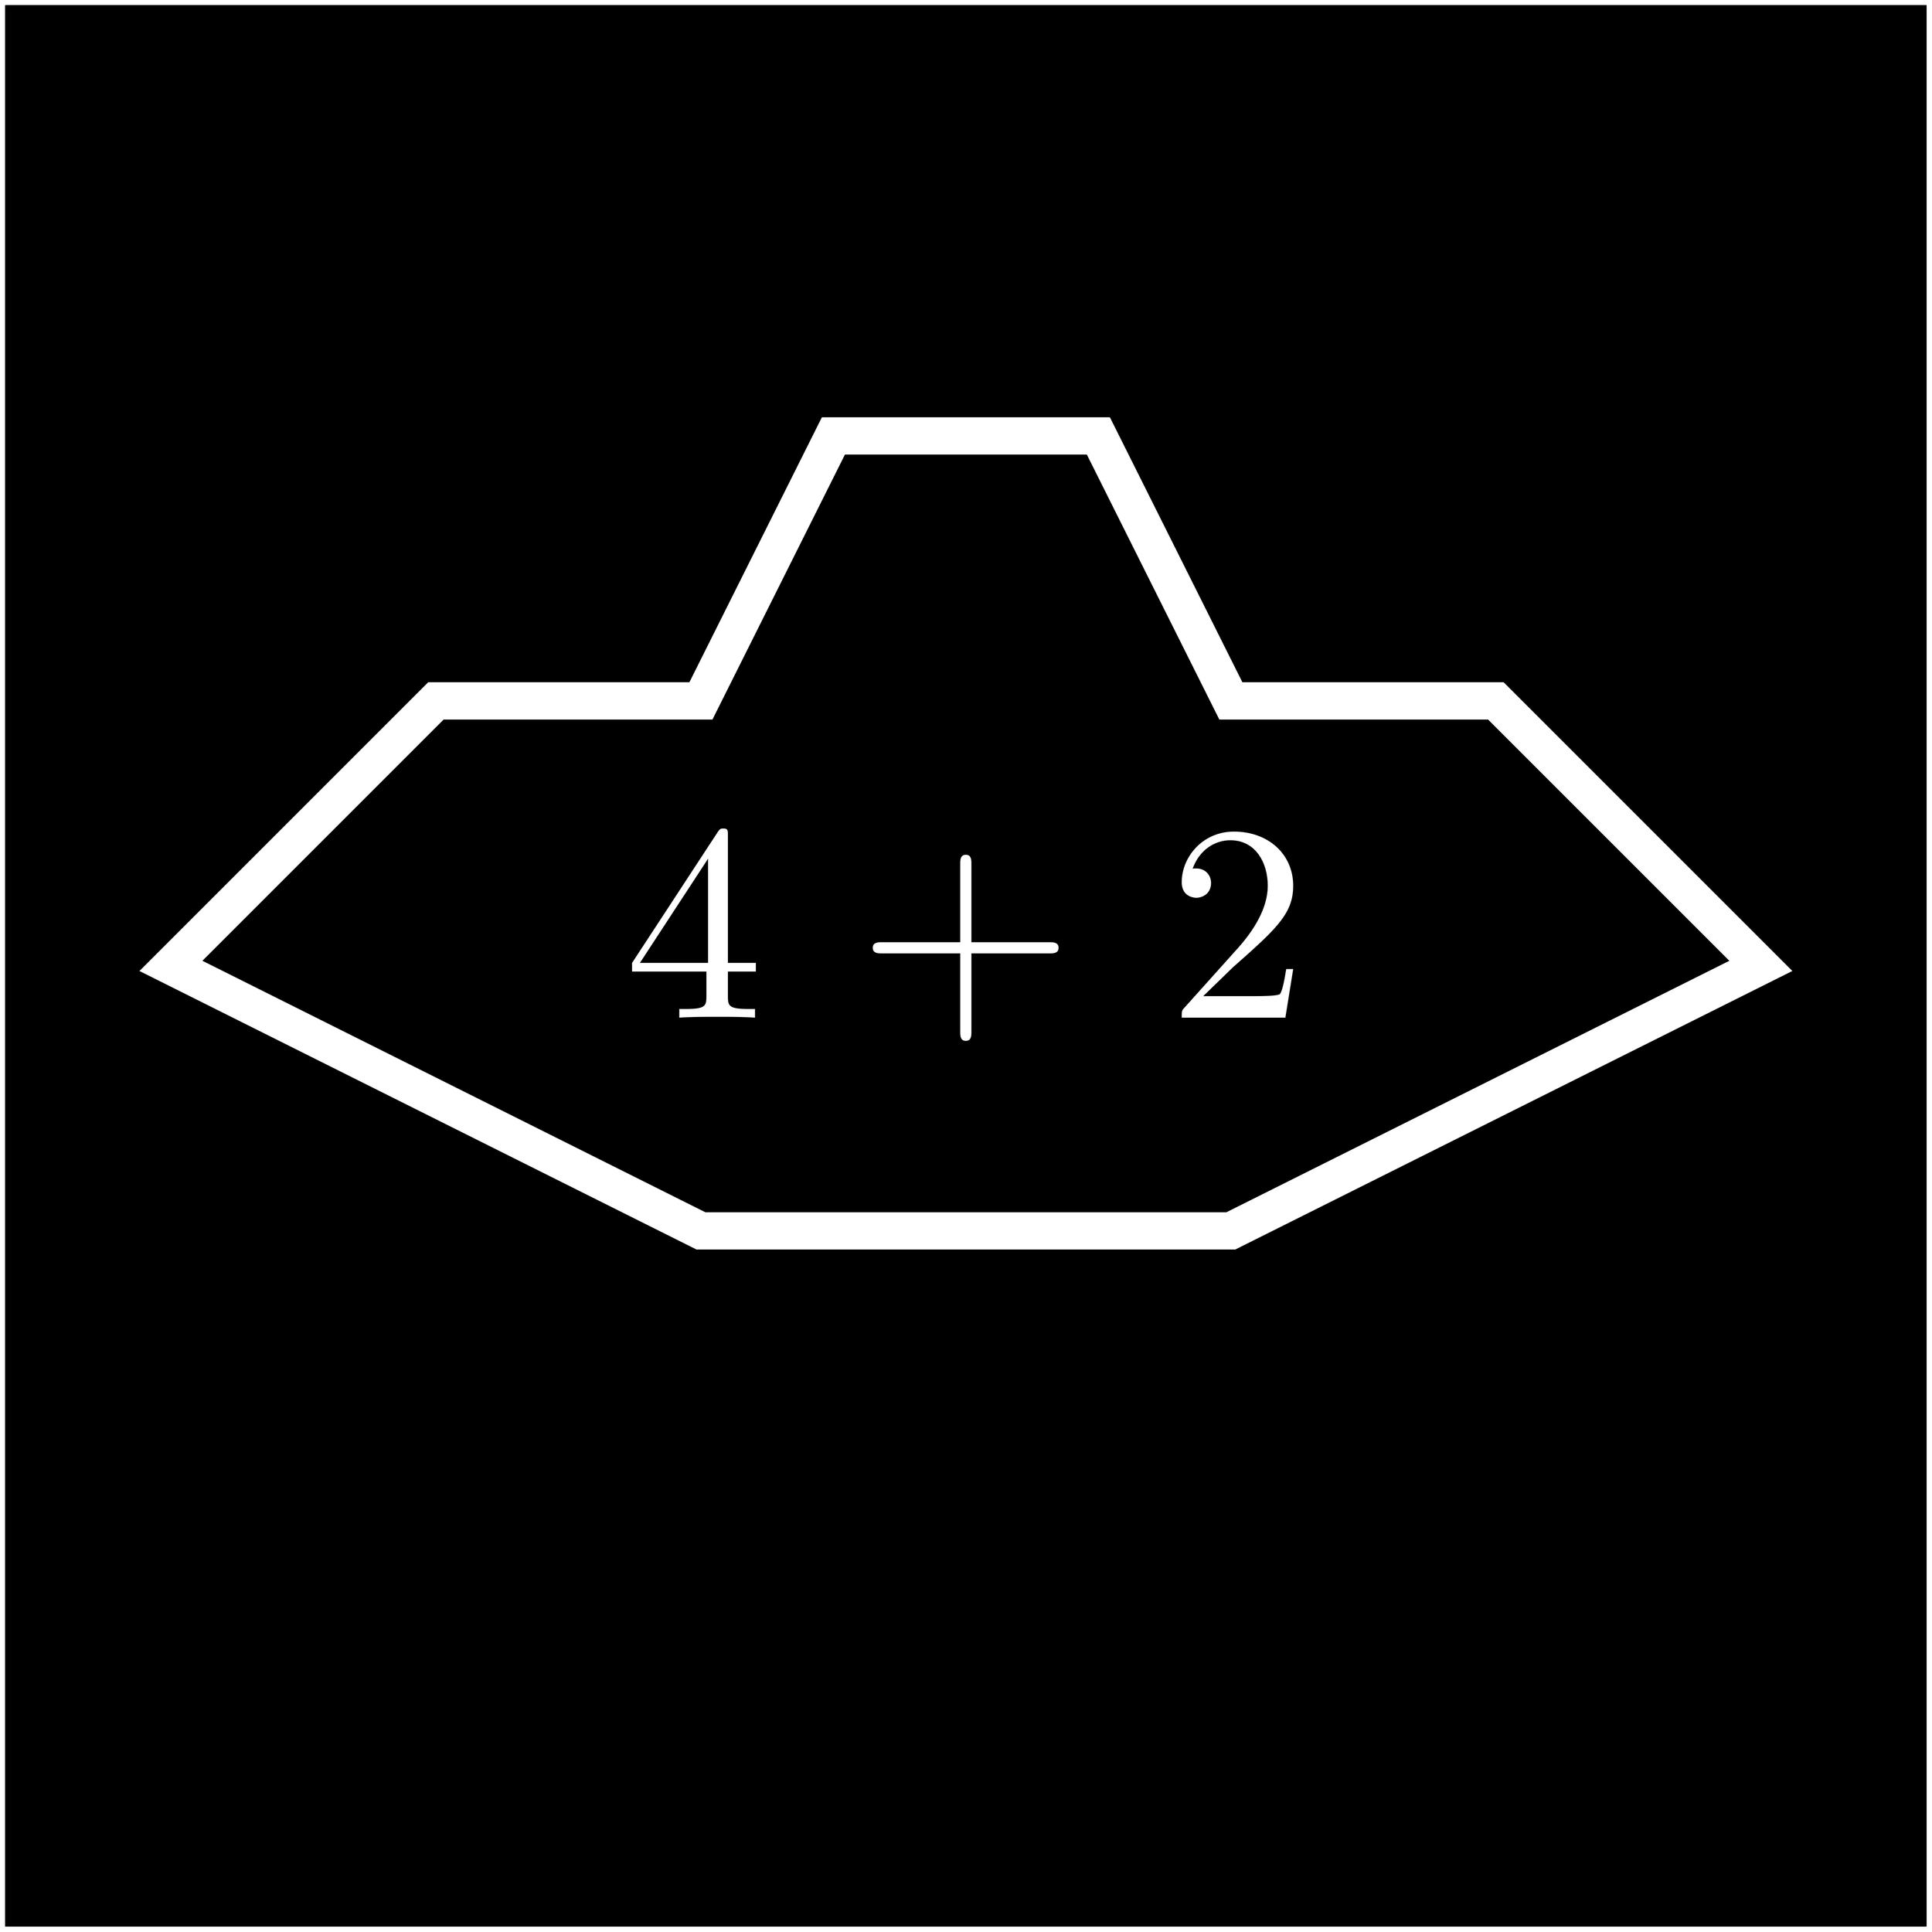
\begin{tikzpicture}[background rectangle/.style= {bottom color=black,top color=black}, show background rectangle]
  %\clip (0,0) circle (35.9662);
  \clip (0,0) circle (36.1);
  \draw[white,line width=40pt] (-10,-10) -- (-30,0) -- (-20,10) -- (-10,10) -- (-5,20) -- (5,20) -- (10,10) -- (20,10) -- (30,0) -- (10,-10) -- cycle;
  \draw[white] (0,1) node[scale=30] {4 + 2};

\end{tikzpicture}

\end{document}
